\chapter{Landau Notation}
%
Die Informatik ist daran interessiert, Algorithmen---die im Alltag zur Anwendung kommen\footnote{Ein bekanntes Beispiel sind hierfür Sortieralgorithmen.}---zu optimieren, um Rechenzeit und Energie zu sparen. Effizientere Algorithmen erlauben ein wirtschaftlicheres Handeln. Wir benötigen daher ein Werkzeug, um Algorithmen bezüglich ihrer Eigenschaften wie Speicherverbrauch und Laufzeit vergleichen zu können.

Bei den nachfolgenden Beispielen sprechen wir von einer Variable $n$. Es ist wichtig zu wissen, wofür dieses $n$ steht, doch ergibt es sich aus dem Kontext oft implizit. Bei einem Sortieralgorithmus wird man mit $n$ die Anzahl der zu sortierenden Elemente beschreiben. Bei der Multiplikation zweier Zahlen wird man die maximale Anzahl der Stellen der beiden Zahlen mit $n$ bezeichnen. Sollte es sich aus dem Kontext nicht eindeutig ergeben, so ist eine textuelle Beschreibung von $n$ sehr wichtig.

Unser neues Werkzeug nennt sich ,,Landau-Notation'', ,,$\mathcal{O}$-Notation''\footnote{In \LaTeX{}  \texttt{\textbackslash mathcal\{O\}} und in Unicode U+039F ``GREEK CAPITAL LETTER OMICRON''} oder engl.~``Big O-Notation''.

\section{2 grundlegende Klassen}
\subsection{Konstante Laufzeiten}
%
\begin{algorithm}[p]
\caption{Subroutine with constant runtime}
\label{algo:constant}
\lstset{language={python}, label={lst:pyconstant}}
\begin{lstlisting}
#!/usr/bin/env python

def function(lst):
    return 0

function([1, 2, 3, 4])
\end{lstlisting}
\end{algorithm}

Der Algorithmus in Funktion~\ref{algo:constant} nimmt eine Liste \textit{array} als Parameter und gibt unabhängig von der Länge des Parameters einen Wahrheitswert zurück. Seine Laufzeit ist damit konstant.

\subsection{Lineare Laufzeiten}
%
\begin{algorithm}[p]
\caption{Subroutine with linear runtime}
\label{algo:linear}
\lstset{language={python}, label={lst:pylinear}}
\begin{lstlisting}
#!/usr/bin/env python

def function(lst):
    for number in lst:
        print(number)
    return 0

function([1, 2, 3, 4])
\end{lstlisting}
\end{algorithm}

Der Algorithmus (Funktion~\ref{algo:linear}) benötigt eine lineare Laufzeit. Der Ablauf der Funktion verrät, dass er über alle Elemente der übergebenen Liste iteriert und damit genau $n$ Schritte benötigt, wenn $n$ die Anzahl der Listenelemente beschreibt. Wird ein $n$ hinzugefügt, benötigt der Algorithmus 1 Zeiteinheit mehr. Es besteht eine \emph{direkte Proportionalität} zwischen $n$ und der Anzahl von Schritten.

\section{Woher $\mathcal{O}$ kommt}
%
Wird ein Algorithmus häufig verwendet, wird es besser sein einen Algorithmus mit konstanter Laufzeit zu wählen. Wir können dann versichern, dass unabhängig von der Größe der Eingabedaten (zB Text des Benutzers in einem Webbrowser) der Algorithmus jeweils mit der selben Laufzeit zum Ergebnis kommt. Dies wird in der Praxis relevant, sobald Inputdaten beliebige Größen besitzen dürfen.
%
\begin{table}
 \begin{center}
  \begin{tabular}{ccc}
   $n$ & Schritte für $f_1$ & Schritte für $f_2$ \\
  \hline
   1  & 1                  & 1 \\
   2  & 1                  & 2 \\
   3  & 1                  & 3 \\
   100 & 1                 & 100 \\
   $10^6$ & 1              & $10^6$ \\
 \hline
  \end{tabular}
  \caption{Zwei Algorithmen, deren Laufzeit mit $f_1(n) = 1$ und $f_2(n) = n$ beschrieben werden können, im Vergleich}
 \end{center}
\end{table}

Wir führen nun die $\mathcal{O}$-Notation ein und untersuchen, ob eine der beiden Funktionen ,,größer'' ist als die andere. ,,Größer'' bedeutet mathematisch wir finden eine Schranke $g(n)$ für eine Funktion $f(n)$, die stets größere Werte liefert als $f(n)$. In diesem Fall sprechen wir von einer ,,oberen Schranke'' und uns interessiert das asymptotische Verhalten.

Wir überlegen uns intuitiv folgende Definition: Eine Funktion $g(n)$ ist die obere Schranke von $f(n)$, wenn\dots
\[
  \forall n \in \mathbb{N}: f(n) \leq g(n)
\]

Beachte, dass wir hier die Einschränkung treffen, dass wir von positiven Zahlen sprechen. Ein Algorithmus mit negativer Laufzeit ist nur theoretisch vorhanden\footnote{Mit der bisherigen Definition werden wir feststellen, dass $f_2$ keine obere Schranke für $f_1$ bei negativen $n$ darstellt. Wir führen jedoch später ein Konstrukt ein, welches $f_2$ zu einer oberen Schrank macht.} und wird nicht von uns behandelt. \\
Im Vergleich von $f_1(n) = 1$ und $f_2(n) = n$ können wir $f_1$ als $f(n)$ und $f_2$ als $g(n)$ einsetzen. Wir stellen fest, dass für ein beliebiges $n$ das Ergebnis der Funktion $g(n)$ ein größeres Ergebnis liefert. $f_2$ ist eine obere Schranke von $f_1$.

Wir vergleichen noch zwei andere Funktionen:
\[
   f_1(n) = 42   \hspace{40pt}  f_2(n) = \pi \cdot n
\]
Wir erhalten für $n = 2$ bei $f_1(2) = 42$ und bei $f_2(2) \approx 6,283$. Es ist irgendwie unbefriedigend, dass $f_2$ \emph{keine} obere Schranke von $f_1$ ist, da die Werte von $f_1$ kleiner als jene von $f_2$ für niedrige $n$ sind. Es ist doch erkennbar, dass ab einen gewissen $n$ die Funktion $f_2$ wesentlich stärker wächst. Daher erweitern wir unsere Definition um einen Mindestwert, ab dem diese Kleiner-Gleich-Relation erst gelten muss.

Wir betrachten eine Funktion (die zB eine Laufzeit beschreibt). Es sei folgende Definition gegeben:
\[
  \On{g(n)} = \{ f(n) \mid \exists n_0 \in \mathbb{N}, \:\forall n \geq n_0: f(n) \leq g(n) \}
\]
Diese Definition erfüllt, was wir erreichen wollen. Für sehr große $n$ vergleichen wir die Algorithmen und beobachten welche Funktion schneller wächst.

Wir treffen jedoch noch eine Entscheidung: Algorithmen mit linearer Laufzeit sind nicht sehr attraktiv. Die Information ,,die Funktion wächst linear'' ist wichtig, aber ob sie mit dem Faktor $2$ oder $3$ wächst, bezeichnen wir als irrelevant. Auch wenn $f_1(n) = 2n$ langsamer wächst als $f_2(n) = 3n$ so sind sie doch sehr ähnlich. Wir möchten definieren, dass Funktionen mit konstanten Faktoren in der selben Klasse liegen. Wir erweitern unsere Definition ein letztes Mal und führen dazu einen Faktor $c$ ein:
\[
   \On{g(n)} = \{ f(n) \mid \exists c \in \mathbb{R}^+, n_0 \in \mathbb{N},
                  \:\forall n \geq n_0: f(n) \leq c \cdot g(n) \}
\]
%
Diese Definition ist unser formaler Unterbau zur Betrachtung der Landau-Notation.

\section{Landau-Notation verallgemeinert}
%
Wobei wir hier in unserem Fall von Laufzeiten sprechen, behandelt die Landau-Notation allgemein asymptotisches Verhalten von Funktionen. Der zweite große Anwendungsbereich der Landau-Notation in der Informatik ist der Speicherverbrauch. Wie viel mehr Speicher brauche ich bei größeren Eingabedaten?

Abseits von der oberen Schranke $\mathcal{O}$ gibt es auch untere Schranken $\Omega$. Bei dieser wird im Gegensatz zur Definition von $\mathcal{O}$ das $\leq$ gegen ein $\geq$ getauscht. Diese Schranke wird in diesem Dokument nicht weiter behandelt.

Es existiert auch die Definition der exakten Schranke $\Theta$, welche weiter unten im Dokument betrachtet wird.

\subsection{Die Landau-Notation visualisiert}
%
\begin{figure}[p]
 \begin{center}
  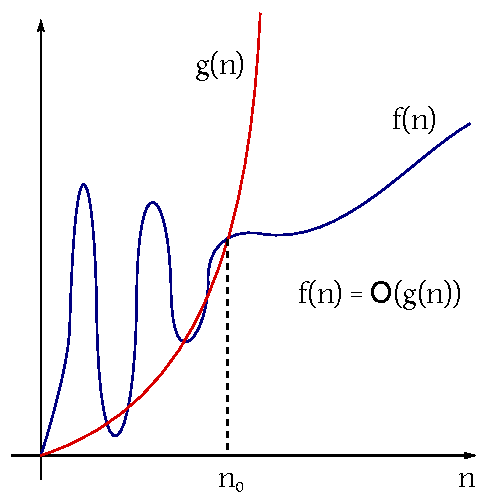
\includegraphics{img/upper_bound.pdf}
  \caption{$g(n)$ bildet eine obere Schranke von $f(n)$}
  \label{fig:upper}
 \end{center}
\end{figure}
\begin{figure}[p]
 \begin{center}
  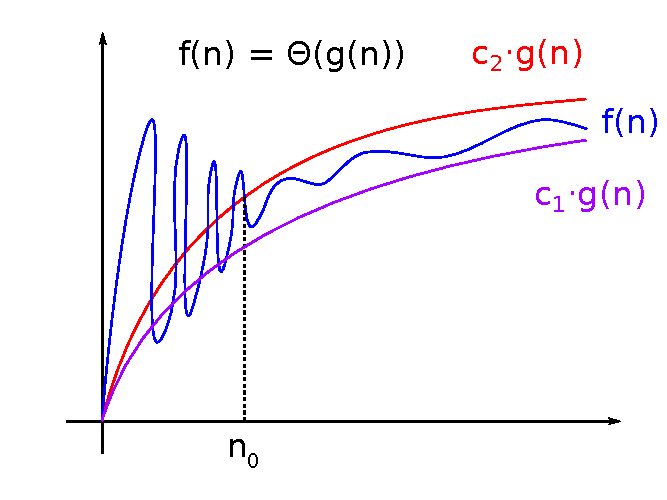
\includegraphics{img/exact_bound.pdf}
  \caption{$g(n)$ bildet eine exakte Schranke von $f(n)$}
  \label{fig:exact}
 \end{center}
\end{figure}

\paragraph{Abbildung~\ref{fig:upper}}
Gegeben sei eine beliebige Funktion $f(n)$ mit der oberen Schranke $g(n)$. Wir können nun ein beliebiges $n_0$ definieren, wobei ab diesem $n_0$ jeder Wert von $g(n)$ größer ist als der Wert von $f(n)$.

\paragraph{Abbildung~\ref{fig:exact}}
Gegeben sei eine beliebige Funktion $f(n)$ mit der exakten Schranke $g(n)$. Wir können nun ein beliebiges $n_0$ definieren, ab dem wir versichern können, dass $f(n)$ zwischen zwei Funktionen $g(n)$ liegt. Dabei kann das $g(n)$ durch einen beliebigen Faktor skaliert werden.

\subsection{Algorithmen-Sequenzen}
%
\begin{algorithm}
\caption{Subroutine with sequence of sub-algorithms}
\label{algo:sequence}
\lstset{language={python}, label={lst:pyseq}}
\begin{lstlisting}
#!/usr/bin/env python

def function(lst):
    for i in range(int(number)):
        print(i)
    print(lst)
    return 0

function([1, 2, 3, 4])
\end{lstlisting}
\end{algorithm}
%
Gegeben sei ein Algorithmus, welcher in zwei Teilbereiche geteilt werden kann (Funktion~\ref{algo:sequence}).
Einerseits haben wir eine Iteration, welche auf die Laufzeitfunktion $f_1(n) = n$ deutet.
Folgend haben wir einen Algorithmus, welcher die Liste ausgibt und $f_2(n) = 1$ Laufzeit besitzt.
Wie verhält sich jetzt die gesamte Laufzeit des Algorithmus? Dazu können wir die Rechenregeln für $\mathcal{O}$-Notation beachten.
%
\[
  \On{f(n)} + \On{g(n)} = \On{\max\left(f(n), g(n)\right)}
\] \[
  \On{f(n)} \cdot \On{g(n)} = \On{f(n) \cdot g(n)}
\]
%
Die erste Regel besagt, dass bei sequentieller Betrachtung der Algorithmen die am stärksten zu wachsende Funktion die asymptotische Schranke vorgibt. Die zweite Regel beschreibt eine verschachtelte Ausführung wie in Funktion~\ref{algo:nested}. Für Funktion~\ref{algo:sequence} berechnen wir:
%
\[
  \On{n} + \On{1} = \On{\max\left(n, 1\right)} = \On{n}
\]
Für die Funktion~\ref{algo:nested} gilt:
\[
  \On{n} \cdot \On{1} = \On{n \cdot 1} = \On{n}
\]
%
Wir merken uns also: Wir müssen immer alle Elemente des Algorithmus betrachten, um die Gesamtlaufzeit angeben zu können.

\begin{algorithm}
\caption{Subroutine with nested algorithms}
\label{algo:nested}
\lstset{language={python}, label={lst:pynested}}
\begin{lstlisting}
#!/usr/bin/env python

def function(lst):
    for i in range(int(number)):
        print(i)
        print(lst)
    return 0

function([1, 2, 3, 4])
\end{lstlisting}
\end{algorithm}
%
\section{Die Unschärferelation}
%
\begin{algorithm}
\caption{Subroutine with runtime square rooted to input value}
\label{algo:sqrt}
\lstset{language={python}, label={lst:pyruntimesquared}}
\begin{lstlisting}
#!/usr/bin/env python

import math

def function(lst):
    return math.sqrt(len(lst))

function([1, 2, 3, 4])
\end{lstlisting}
\end{algorithm}
%
Wir betrachten den Algorithmus in Funktion~\ref{algo:sqrt}. Wir haben hier ein Problem, wenn wir die Schlussfolgerungen des vorigen Kapitels beachten. Wir benutzen die Funktion \verb=math.sqrt=, welche uns die Quadratwurzel einer Länge der Inputmenge \textit{lst} zurückliefert. Wir wissen jedoch nicht welche Laufzeit \verb=math.sqrt= besitzt.

Die Funktion wird über mehrere Abstraktionsebenen schlussendlich eine Maschinencode-Instruktion aufrufen, welche uns das Ergebnis maschinennah ermittelt. Die Frage ist jedoch mit welcher Laufzeit dieses Ergebnis ermittelt werden kann. Handelt es sich nur um einen Lookup in einer Tabelle, könnte es sich um $\On{1}$ handeln. Umgekehrt sind aber auch Algorithmen mit $\On{n}$ Zeitkomplexität bekannt. Ebenso habe ich verschwiegen, welche Komplexität ein return-Statement besitzt. Es scheint als ob wir hier Algorithmen gar nicht untersuchen können ohne die gesamte Maschine zu betrachten.

Die Aussage des letzten Absatzes ist fehlerfrei und begründet die Genialität der Turingmaschine. Die Turingmaschine bietet uns ein universales Konzept mit dem wir die Laufzeit $1:1$ mit der Anzahl der ausgeführten Schritte beobachten können. Sie dient uns als Referenzmaschine auf der wir all unsere Algorithmen untersuchen können. Daher ist die Turingmaschine ein elementares Konzept der theoretischen Informatik.
%
\section{Weitere Klassen von Funktionen}
%
Zum dritten Mal in diesem Dokument wird der Begriff ,,Klasse'' verwendet. Wir besitzen jedoch noch keine Definition einer ,,Klasse''. Dieser Begriff ist etwas komplizierter, jedoch möchten wir ihn kurz formal definieren:
Zwei Funktionen liegen in der selben Klasse, wenn sie gegenseitig eine exakte Schranke der anderen Funktion sind. Die Definition der exakten Schranke ist gegeben als:
\[
  \On{g(n)} = \{ f(n) \mid \exists c_1, c_2 \in \mathbb{R}^+, n_0 \in \mathbb{N},
                 \forall n \geq n_0: c_1 \cdot g(n) \leq f(n) \leq c_2 \cdot g(n) \}
\]
%
Wir verwenden also einen Faktor $c_1$ um die Schranke $g(n)$ nach unten zu skalieren und eine entsprechende untere Schranke zu erhalten. Genauso können wir $g(n)$ mit $c_2$ nach oben skalieren, um eine obere Schranke zu erhalten.

Liegen jetzt $f_1(n) = 2n$ und $f_2(n) = 3n$ in der selben Klasse? Wir beobachten, ob sie gegenseitig exakte Schranken sind. Wir betrachten die mathematische Definition:
\[
  \On{3n} = \{ 2n \mid \exists c_1, c_2 \in \mathbb{R}^+, n_0 \in \mathbb{N},
              \forall n \geq n_0: c_1 \cdot 3n \leq 2n \leq c_2 \cdot 3n \}
\] \[
  \On{2n} = \{ 2n \mid \exists c_3, c_4 \in \mathbb{R}^+, n_0 \in \mathbb{N},
              \forall n \geq n_0: c_3 \cdot 2n \leq 3n \leq c_4 \cdot 2n \}
\]
%
Ohne große Ausführungen zu machen, setzen wir $c_1 = \frac13$, $c_2 = 1$, $c_3 = 1$ und $c_4 = 2$, um alle mathematischen Ausdrücke zu einer wahren Aussage zu bewegen und wir sehen, dass beide Funktionen exakte Schranken zueinander sind.
%
\subsection{Logarithmische Funktionen}
%
Algorithmen mit konstanter Laufzeit werden durch Unabhängigkeit von der Eingabemenge begründet.
Die Iteration in Abhängigkeit der Eingabemenge definiert die Klasse der Algorithmen mit linearer Laufzeit.
Eine weitere Klasse wird durch logarithmisches Verhalten begründet.
%
\subsubsection{Die Binärsuche}
%
Die Binärsuche (Funktion~\ref{algo:binsearch}) ist der bekannteste Vertreter der logarithmischen Algorithmen. Als Parameter übergeben wir 2 Werte: Eine aufsteigend sortierte Liste mit Zahlen und eine Zahl. Retourniert werden soll der Index der Zahl in der Liste. Der Algorithmus setzt einen Index in die Mitte der Liste. Ist der Wert in der Mitte größer, wird der Suchbereich auf den linken Teil beschränkt. Ist der Wert kleiner, suchen wir den Wert rechts. Der Suchbereich wird durch \verb=width= definiert. \verb=index= beinhaltet den Index des betrachteten Werts in Funktion~\ref{algo:binsearch}.

Wir möchten das Zeitverhalten des Algorithmus ermitteln. Dabei stellt sich heraus, dass der Algorithmus schneller ist als den Wert mit allen Werten zu vergleichen ($\On{n}$) und langsamer ist als eine Konstante ($\On{1}$). Wir teilen den Suchbereich immer durch zwei. Wir erhalten damit einen Binärbaum der Höhe $\log_2{n}$ in dem genau 1 Wert gesucht wird.

\subsubsection{Die Äquivalenz der logarithmischen Klassen}
%
Logarithmische Funktionen mit unterschiedlicher Basis liegen alle in der selben Klasse. Wir können dies beweisen, indem wir es als formalen Beweis durchführen. Wir zeigen, dass $f_1(n) = \log_2(n)$ eine exakte Schranke von $f_2(n) = \log_3(n)$ und vice versa ist.
\[
  \On{\log_2{n}} \stackrel{?}{=} \On{\log_3{n}}
\] \[
  \log_2{n} = \frac{\log{n}}{\log{2}}
\] \[
 \Theta(\log_3{n}) \stackrel{?}{=} \{ \log_2{n} \mid \exists c_1, c_2 \in \mathbb{R}^+, n_0 \in \mathbb{N},
                      \forall n \geq n_0: c_1 \cdot \log_3{n} \leq \log_2{n} \leq c_2 \cdot \log_3{n} \}
\] \[
  c_1 \cdot \frac{\log{n}}{\log{3}} \leq \frac{\log{n}}{\log{2}} \leq c_3 \cdot \frac{\log{n}}{\log{3}}
\] \[
  c_1 \cdot \frac{1}{\log{3}} \leq \frac{1}{\log{2}} \leq c_2 \cdot \frac{1}{\log{3}}
\] \[
  3.3219 \cdot c_1 \leq 2.0959 \leq 3.3219 \cdot c_2
\] \[
  \text{Wahre Aussage mit } \{c_1 = \frac12, c_2 = 1\}
\] \[
  \Rightarrow \log_2(n) \in \Theta(\log_3(n))
\] \[
  \Theta(\log_2{n}) \stackrel{?}{=} \{ \log_3{n} \mid \exists c_1, c_2 \in \mathbb{R}^+, n_0 \in \mathbb{N},
                      \forall n \geq n_0: c_1 \cdot \log_2{n} \leq \log_3{n} \leq c_2 \cdot \log_2{n} \}
\] \[
  \Theta(\log_2{n}) = \{ \log_3{n} \mid \exists c_1, c_2 \in \mathbb{R}^+, n_0 \in \mathbb{N},
                      \forall n \geq n_0: c_1 \cdot \frac{\log{n}}{\log{2}} \leq \frac{\log{n}}{\log{3}} \leq c_2 \cdot \frac{\log{n}}{\log{2}} \}
\] \[
  c_1 \cdot \frac{1}{\log{2}} \leq \frac{1}{\log{3}} \leq c_2 \cdot \frac{1}{\log{2}}
\] \[
  2.0959 \cdot c_1 \leq 3.3219 \leq 2.0959 \cdot c_2
\] \[
  \text{Wahre Aussage mit } \{c_1 = 1, c_2 = 2\}
\] \[
  \Rightarrow \log_3(n) \in \Theta(\log_2(n))
\]
%
Obwohl die Frage sich auf $\mathcal{O}$ (obere Schranke) bezogen hat und wir $\Theta$ (exakte Schranke) bewiesen, ist der Beweis vollständig, da eine exakte Schranke die obere Schranke impliziert:
\[
   f(n) \in \Theta(g(n)) \Leftrightarrow f(n) \in \On{g(n)} \land f(n) \in \Omega(g(n))
\]

Im Übrigen haben wir bei diesem Beweis zum ersten Mal gesehen, dass die Notation $f(n) = \On{g(n)}$ äquivalent zur Notation $f(n) \in \On{g(n)}$ ist. Werden \emph{zwei Klassen} gegenüber gestellt, so verwendet man Symbole der Mengenlehre.
%
\begin{algorithm}
\caption{Binary search algorithm}
\label{algo:binsearch}
\lstset{language={python}, label={lst:pybinsearch}}
\begin{lstlisting}
import math

def binary_search(n, search):
    index = len(n) / 2
    width = len(n) / 2
    while True:
        if n[index] == search:
            return index
        if width == 0:
            raise KeyError("Value not in list")

        elif n[index] > search:
            index -= (width + 1) / 2
        else:
            index += (width + 1) / 2

        width /= 2

binary_search([1, 2, 3, 4], 2)
\end{lstlisting}
\end{algorithm}
%
\subsection{Polynomielle Funktionen der Form $n^k$}
%
Funktionen der Form $f(n) = n^k$ mit $k \in \mathbb{R}^+$ treten auch häufig auf. Ein typischer Algorithmus mit solch einer Struktur ist eine verschachtelte Schleife. Liegt in einer Schleife über alle Inputwerte eine Schleife über alle Inputwerte vor, wird pro Wert die gesamte Liste iteriert. Eine solche Funktion wächst ziemlich schnell, doch ist es wieder interessant, ob Funktionen mit unterschiedlichem $k$ in der selben Klasse liegen. Wir müssen uns wieder auf die formale Ebene bewegen und zeigen, dass etwa $n^3$ eine exakte Schranke von $n^2$ ist:

\[
 \Theta(n^3) \stackrel{?}{=} \{ n^2 \mid \exists c_1, c_2 \in \mathbb{R}^+, n_0 \in \mathbb{N},
                                \forall n \geq n_0: c_1 \cdot n^3 \leq n^2 \leq c_2 \cdot n^3 \}
\] \[
  c_1 \cdot n^3 \leq n^2 \leq c_2 \cdot n^3
\] \[
  \log{(c_1)} + 2\cdot\log{n} \leq 3\cdot\log{n} \leq \log{(c_2)} + 2\cdot\log{n}
\] \[
  \frac{\log{c_1}}{\log{n}} + 2 \leq 3 \leq \frac{\log{c_2}}{\log{n}} + 2
\]
Das $n$ liegt unter dem Bruch und definiert damit mit größerem $n$ einen kleinen Gesamtwert. Wir schaffen es nicht ein beliebiges $n_0$ zu finden für das für alle größeren $n$ die Relation $\frac{\log{c_1}}{\log{n}} + 2 \leq 3$ gilt. Der Beweis ist damit gescheitert. Wir halten somit fest, dass alle Funktionen unterschiedlicher Hochzahl eine eigene Klasse bilden.
%
\subsection{Exponentielle Funktionen}
%
Exponentialfunktionen besitzen eine Struktur wie $k^n$. Wieder es interessiert uns, ob alle Exponentialfunktionen unterschiedlicher Basis in eine Klasse von Funktionen gehören. Wir vergleichen ${42}^n$ mit $2^n$ und legen damit wieder unsere exakte Schranke an:
\[
  \Theta({42}^n) \stackrel{?}{=} \{ 2^n \mid \exists c_1, c_2 \in \mathbb{R}^+, n_0 \in \mathbb{N},
                                    \forall n \geq n_0: c_1 \cdot {42}^n \leq 2^n \leq c_2 \cdot {42}^n \}
\] \[
  c_1 \cdot {42}^n \leq 2^n \leq c_2 \cdot {42}^n
\] \[
  \log(c_1) + n\cdot\log{42} \leq n\log{2} \leq \log(c_2) + n\cdot\log{42}
\] \[
  \frac{\log(c_1)}{n} + \log{42} \leq \log{2} \leq \frac{\log(c_2)}{n} + \log{42}
\]
Wir haben selbiges Problem wie bei vorigem Beweis: Diese Relation ist nicht für konstante $c_1$ und $c_2$ und beliebig große $n$ erfüllt. Daher begründen alle Exponentialfunktionen mit unterschiedlicher Basis eigene Klassen.

\subsection{Exponentielle Funktion mit konstanten Summanden in der Hochzahl}
%
Wie sieht es mit $3^n$ gegenüber $3^{n+1}$ aus? Liegen die beiden Funktionen in der selben Klasse?
Wieder muss die exakte Schranke vice versa gezeigt werden:
%
\[
  \Theta(3^n) \stackrel{?}{=} \{ 3^{n+1} \mid \exists c_1, c_2 \in \mathbb{R}^+, n_0 \in \mathbb{N},
                                 \forall n \geq n_0: c_1 \cdot {3}^n \leq 3^{n+1} \leq c_2 \cdot {3}^n \}
\] \[
  c_1 \cdot 3^n \leq 3^n \cdot 3 \leq c_2 \cdot {3}^n
\]% \[
%  \log(c_1) + n\cdot\log{3} \leq \log{3} + n\cdot\log{3} \leq \log(c_2) + n\cdot\log{3}
%\] \[
%  \underbrace{\frac{\log(c_1)}{n\cdot\log{3}} + 1}_{\text{konvergiert gegen 1}} \leq \underbrace{\frac{1}{n} + 1}_{\text{konvergiert gegen 1}} \leq \underbrace{\frac{\log(c_2)}{n\cdot\log{3}} + 1}_{\text{konvergiert gegen 1}}
%\] \[
%  1 \leq 1 \leq 1
%\] \[
%  \Rightarrow \text{Wahre Aussage}
%\]

Mit $c_1 = 3$ und $c_2 = 3$ ergibt sich für beliebiges $n$ ein wahrer Ausdruck. Es gilt somit $3^{n+1} \in \Theta(3^n)$.

\[
  \Theta(3^{n+1}) \stackrel{?}{=} \{ 3^n \mid \exists c_1, c_2 \in \mathbb{R}^+, n_0 \in \mathbb{N},
                                     \forall n \geq n_0: c_1 \cdot {3}^{n+1} \leq 3^n \leq c_2 \cdot 3^{n+1} \}
\] \[
  c_1 \cdot 3^n \cdot 3 \leq 3^n \leq c_2 \cdot 3^n \cdot 3
\]
Mit $c_1 = \frac{1}{3}$ und $c_2 = \frac{1}{3}$ ergibt sich eine wahre Aussage für ein beliebig großes $n$ (daher $3^n \in \Theta(3^{n+1})$).

Da sie exakte Schranken zueinander sind, handelt es sich bei $\On{3^n}$ und $\On{3^{n+1}}$ um die selben Klassen von Funktionen.
%
\subsection{Die Suche nach der langsamst wachsenden Funktion}
%
Wir sprechen von ,,möglichst großem $n$'' und von ,,Wachstum'' sowie ,,oberen Schranken''. Bei der Angabe von Beispielen zum Rechnen findet man jedoch die Frage nach der ,,langsamst wachsenden Funktion''. Wie passen diese Dinge zusammen?

Wir definieren drei Funktionen $f_1(n) = n$, $f_2(n) = 42n$ und $f_3(n) = n^n$. Mithilfe der formalen Definition stellen wir fest, dass die Relationen $f_1 \in \On{n^n}$, $f_2 \in \On{n^n}$ und $f_3 \in \On{n^n}$ gelten. Unzufrieden stellen wir fest, dass jede der betrachteten Funktionen $n^n$ als obere Schranke besitzt. Die Information ,,die Laufzeit fast aller Algorithmen kann mit $\On{n^n}$ abgeschätzt werden'' ist praktisch nicht hilfreich. Aus diesem Grund suchen wir jene Klasse für eine Funktion, in der die Funktion liegt und die im Vergleich zu anderen Klassen am langsamsten wächst.
%
\subsection{Polynomiell vs exponentiell}
%
Abseits der Betrachtung von Klassen gibt es auch Sichtweisen, die Algorithmen in nur 2 Klassen teilen: Polynomielle Funktionen (jene der Struktur $a_1 \cdot n^0 + a_2 \cdot n^1 + a_3 \cdot n^2 + \ldots$) und exponentielle Funktionen. Dabei werden polynomielle Funktionen als ,,effizient'' betrachtet und sind erstrebenswert. Diese Sichtweise begründet die Sichtweise auf ,,Komplexitätsklassen'' in der theoretischen Informatik.
%
\section{Conclusio}
%
Wir betrachten mit der $\mathcal{O}$-Notation verschiedene Klassen von Funktionen, die Attribute wie Laufzeit oder Speicherverbrauch beschreiben. Obwohl sie formal genau definiert ist und ein etabliertes Werkzeug ist, steht die $\mathcal{O}$-Notation auch Kritik\footnote{Suche etwa nach ``Algorithms for the masses''} gegenüber, da sie dem Programmierer nicht jenes Werkzeug zur Verfügung stellt, welches wir immer brauchen (Sprechen wir \emph{immer} von sehr großen $n$? Wird immer sauber definiert, was man mit $n$ bezeichnet?).

In Bezug auf Notation verwenden wir jetzt möglichst einheitliche Notationen für Klassen von Funktionen. Es wäre sinnfrei $\On{3n}$ zu notieren, da es zu $\On{42n}$ äquivalent ist und $\On{n}$ am einfachsten zu schreiben ist. Wir definieren als eine Liste an bekannten Funktionsklassen aufsteigend nach ihrer Komplexität (Tabelle~\ref{tab:classes}).
\begin{table}[ht]
 \begin{center}
  \begin{tabular}{cl}
   Klasse & Beschreibung \\
  \hline
   $\On{1}$ & konstant \\
   $\On{n}$ & linear \\
   $\On{\log{n}}$ & logarithmisch \\
   $\On{n^2}$ & quadratisch \\
   $\On{n^3}$ & kubisch \\
   $\On{n^k}$ & polynomiell $k$-ten Grades (mit $k>3$) \\
   $\On{2^n}$ & exponentiell zur Basis 2 \\
   $\On{3^n}$ & exponentiell zur Basis 3 \\
   $\On{n!}$ & faktoriell \\
  \end{tabular}
  \caption{Funktionenklassen nach $\mathcal{O}$-Notation}
  \label{tab:classes}
 \end{center}
\end{table}

Auf der Basis unseres Verständnisses für die $\mathcal{O}$-Notation, betrachten wir verschiedene Verhältnisse:%
\[
   f_1(n) = 1 \mathspace
   f_2(n) = 42 \mathspace
   f_3(n) = n \mathspace
   f_4(n) = 2n \mathspace
\] \[
   f_5(n) = \log{n} \mathspace
   f_6(n) = \log_2{n} \mathspace
   f_7(n) = n^2 \mathspace
\] \[
   f_8(n) = n^3 \mathspace
   f_9(n) = 3^n \mathspace
   f_{10}(n) = 3^{n+1}
\]
\begin{itemize}
  \item $f_1 \in \On{1}$
  \item $f_2 \in \On{1}$
  \item $f_3 \notin \On{1}$
  \item $f_3 \in \On{n}$
  \item $f_4 \in \On{n}$
  \item $\On{f_3} = \On{f_4}$
  \item $\On{f_1} \subset \On{f_3}$
  \item $f_3 \in \Theta(f_4) \land f_4 \in \Theta(f_3) \Rightarrow \On{f_3} = \On{f_4}$
  \item $f_5 \in \On{\log{n}}$
  \item $f_6 \in \On{\log{n}}$
  \item $f_7 \in \On{n^2}$
  \item $f_8 \notin \On{n^2}$
  \item $f_9 \in \On{3^n}$
  \item $f_9 \notin \On{n}$
  \item $f_9 \notin \On{2^n}$
  \item $f_9 \in \On{f_{10}} \land f_{10} \in \On{f_9}$
  \item $f_{10} \in \On{3^n}$
\end{itemize}

\section{Unbehandelte Themen}
%
\begin{itemize}
  \item Was ist mein $n$ bei mehreren Parametern?
  \item Umgang mit Funktionen die mehrere $n$ definieren?
  \item Wie analysiert man rekursive Funktionen?
  \item Wie stehen obere, untere und exakte Schranken zueinander? Welche Rechenregeln ergeben sich?
\end{itemize}
%
Die Lehrveranstaltungen \coursedaa{}, \coursetcs{} und \coursedaa{} sind Pflichtlehrveranstaltungen der Studiengänge ,,Informatik'', (teilweise) ,,Softwareentwicklung-Wirtschaft'', (teilweise) ,,Telematik'' und (teilweise) ,,(Technische) Mathematik''. Sie behandeln die behandelten und unbehandelten Konzepte tiefergehend.
